\documentclass[]{article}
\usepackage{graphicx}
\usepackage{amssymb}
\usepackage{float}


\title{Using \textit{Maelstrom} to obtain orbital information about KIC 8264492 }
\author{Dillon Hanlon}
\date{\today}

\begin{document}


\maketitle
\begin{abstract}
    Binary and multi star systems have been crucial to our understanding of stellar structure and evolution due to the fact it can provide accurate measurement of stellar masses. This project focuses on using a third-party python software namely \textit{Maelstrom} to model the light curve and produce theoretical light curve data which gives information about the orbit of the binary star. The result model showed a very high correlation with the original light curve data. The optimization parameters obtained were used to produce a simplistic plot of the orbital path of this binary star. 
\end{abstract}
\section{Introduction}
People think of stars as this lonely dot in space that provide light, but
many stars that are in space are actually in a binary system. In fact, binary and even multiple system stars are much more common than single stars by at least a factor of two \cite{guszejnov2017protostellar}. Binary systems however, one or both components can pulsate, meaning that their brightness changes as a function of time. Those that pulsate with some periodicity can provide researchers with a clock also known as a standard candle and help aid their measurements  \cite{murphy2018finding}. Typically the type of stars that appear in these systems are type A to type F main sequence stars \cite{garg2010high}.

Light curves are very useful plots of light intensity (brightness) as a function of time for stars or other astronomical objects for understanding more about that object. The light curve shapes of pulsating stars in a binary systems can give valuable information about the underlying physical processes producing the changes in the brightness (flux). As well, the shape of the light curve can indicate the relative sizes of the stars, relative surface brightness \cite{russell1912determination}. It should be noted that most work in science has many contributions from many different experiments, therefore for astronomical research understanding light curves use information from many observations to get the full details of the object.

\section{Method}
This project focused on using \textit{Maelstrom}, an open source python package that models and analyzes binary light curves with a pulsating component. For this project the celestial object in study is KIC 8264492, a binary star system with a $\delta$ Sct star component located in the field of the open cluster NGC 6866, 3900 light years away, with a mass of 1.87 $M_{\odot}$ and a temperature of $T_{eff} = 7992$K \cite{balona2013pulsation,shibahashi2015fm}.

This project focused on using \textit{Maelstrom}, an open source python package that models and analyzes binary light curves with a pulsating component. For this project the celestial object in study is KIC 8264492, a binary star system with a $\delta$ Scuti star component located in the field of the open cluster NGC 6866, 3900 light years away, with a mass of 1.87 $M_{\odot}$ and a temperature of $T_{eff} = 7992$K \cite{balona2013pulsation,shibahashi2015fm}. 

\begin{figure}[H]
    \centering
    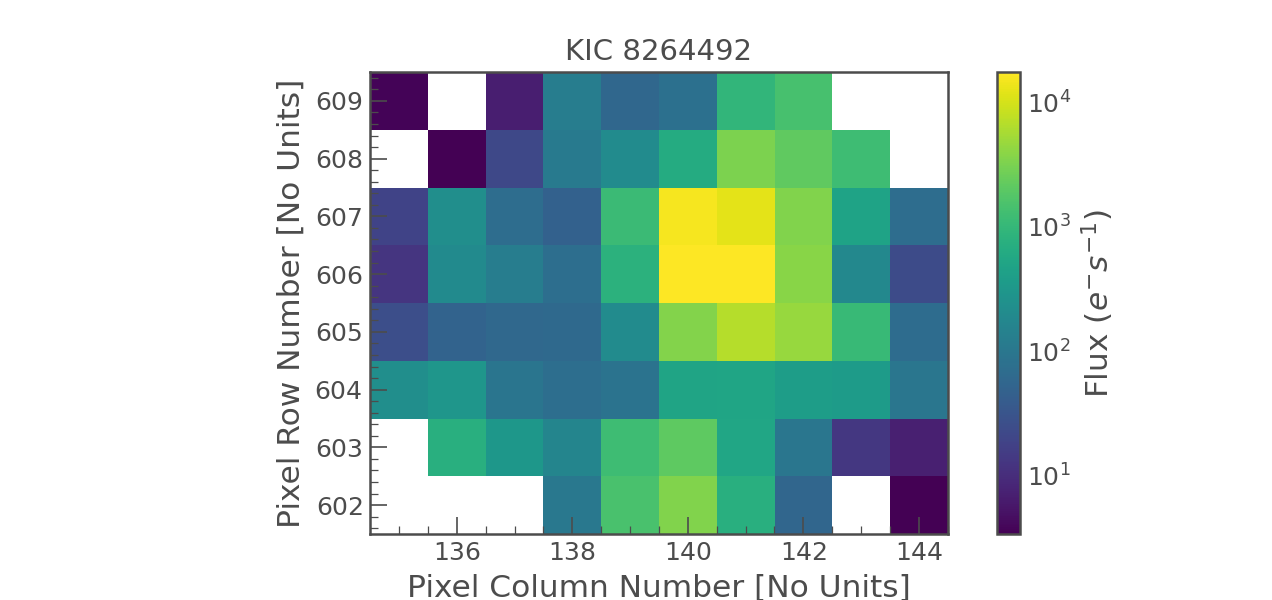
\includegraphics[width=1\linewidth]{Recover_Binary.pdf}
      \caption{Need new caption}
      \label{fig:Recover_Binary}
    \end{figure}


A python module \textit{lightkurve} was used initially to get a pixel image of the pulsating star.  As can be seen from Fig \ref{fig:Recover_Binary} there is an intense region near the center of this image with flux on the order of$\sim$ 10$^4 electrons/second$ which represents the star of interest. \textit{Maelstrom} will forward model the orbit where a light curve is generated from the orbital parameters. How this works is by fitting the phase variation ($\tau$) at each point in the light curve or mathematically;
\begin{equation}
    y(t) = \sum_{j = 1}^{J} [A_j \cos(\omega_j (t - \tau)) + B_j \sin(\omega_j (t - \tau) ]
\end{equation}
\noindent
The light curve for the binary star used in this project can be seen in Fig \ref{fig:Lightcurve}. The module \textit{lightkurve} subtracts 2454844 days which is the Kepler zero time from the time data. Therefore all times are reported in Barycentric Kepler Julian Date (BKJD), doing this corrects for differences in the earths position with respect to the center of the solar system \cite{Eastman_2010}. This light curve data will then be used in \textit{Maelstrom} to produce information about the star.

\begin{figure}[H]
    \centering
    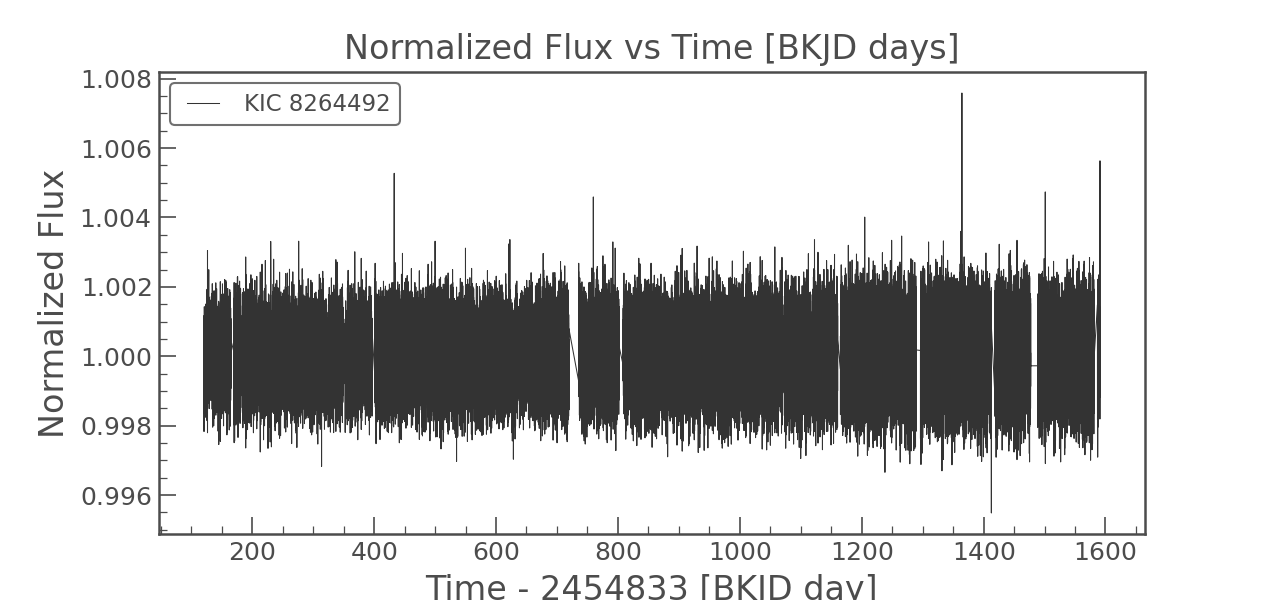
\includegraphics[width=1\linewidth]{Lightcurve.pdf}
      \caption{Need new caption}
      \label{fig:Lightcurve}
\end{figure}


\section{Results}
After the light curve has been passed into \textit{Maelstroms} a forward modelling algorithm begins. This models the light curve data and optimizes its orbital parameters and produces a new theoretical fit for these parameters. Fig \ref{fig:timedelay} shows the original light curve data (from Fig \ref{fig:Lightcurve}) fitted with an theoretical light curve with optimized parameters.

\begin{figure}[H]
    \centering
    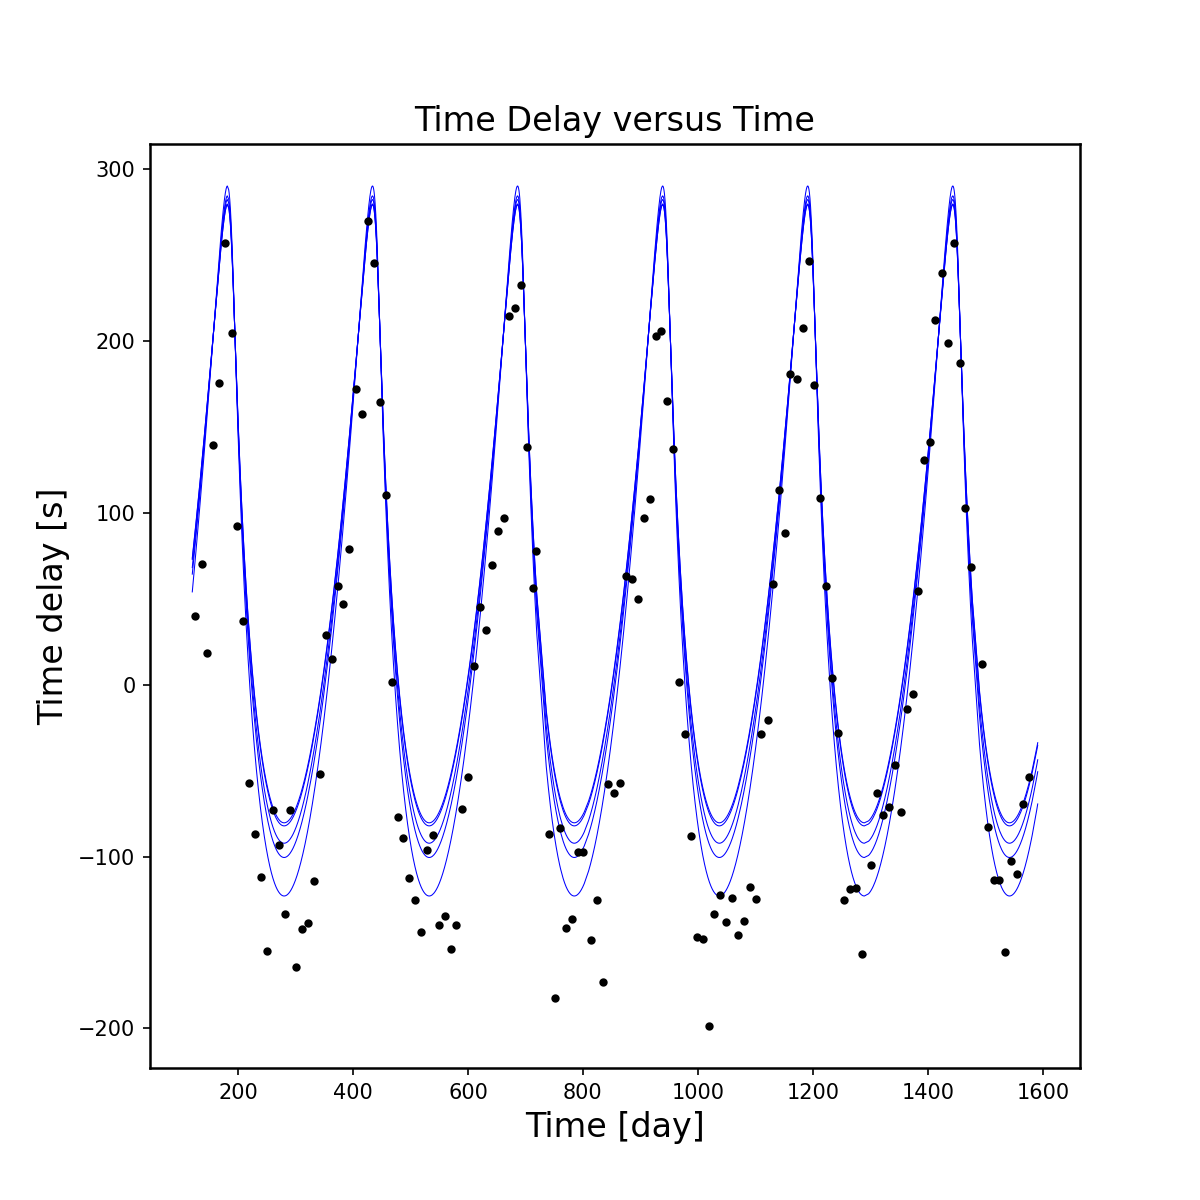
\includegraphics[width=1\linewidth]{time_delay.pdf}
      \caption{Need new caption}
      \label{fig:timedelay}
\end{figure}

The optimized parameters are shown in Table 

\begin{tabular}{c|c}
\hline
    Period  & 2  \\
    Semi-Major Axis & 4\\
    Eccentricity & 6\\
    Orbital Period & \\
    Oscillation Modes & \\
\end{tabular}

\noindent
From these parameters it is possible to make an estimate of the shape of the elliptical orbit for this star. Knowing that the semi-minor axis is related to the semi-major axis by a factor of $1/2$, then it is possible to make a simplistic model of the orbit as shown in Fig \ref{fig:Orbit}

\begin{figure}[H]
    \centering
    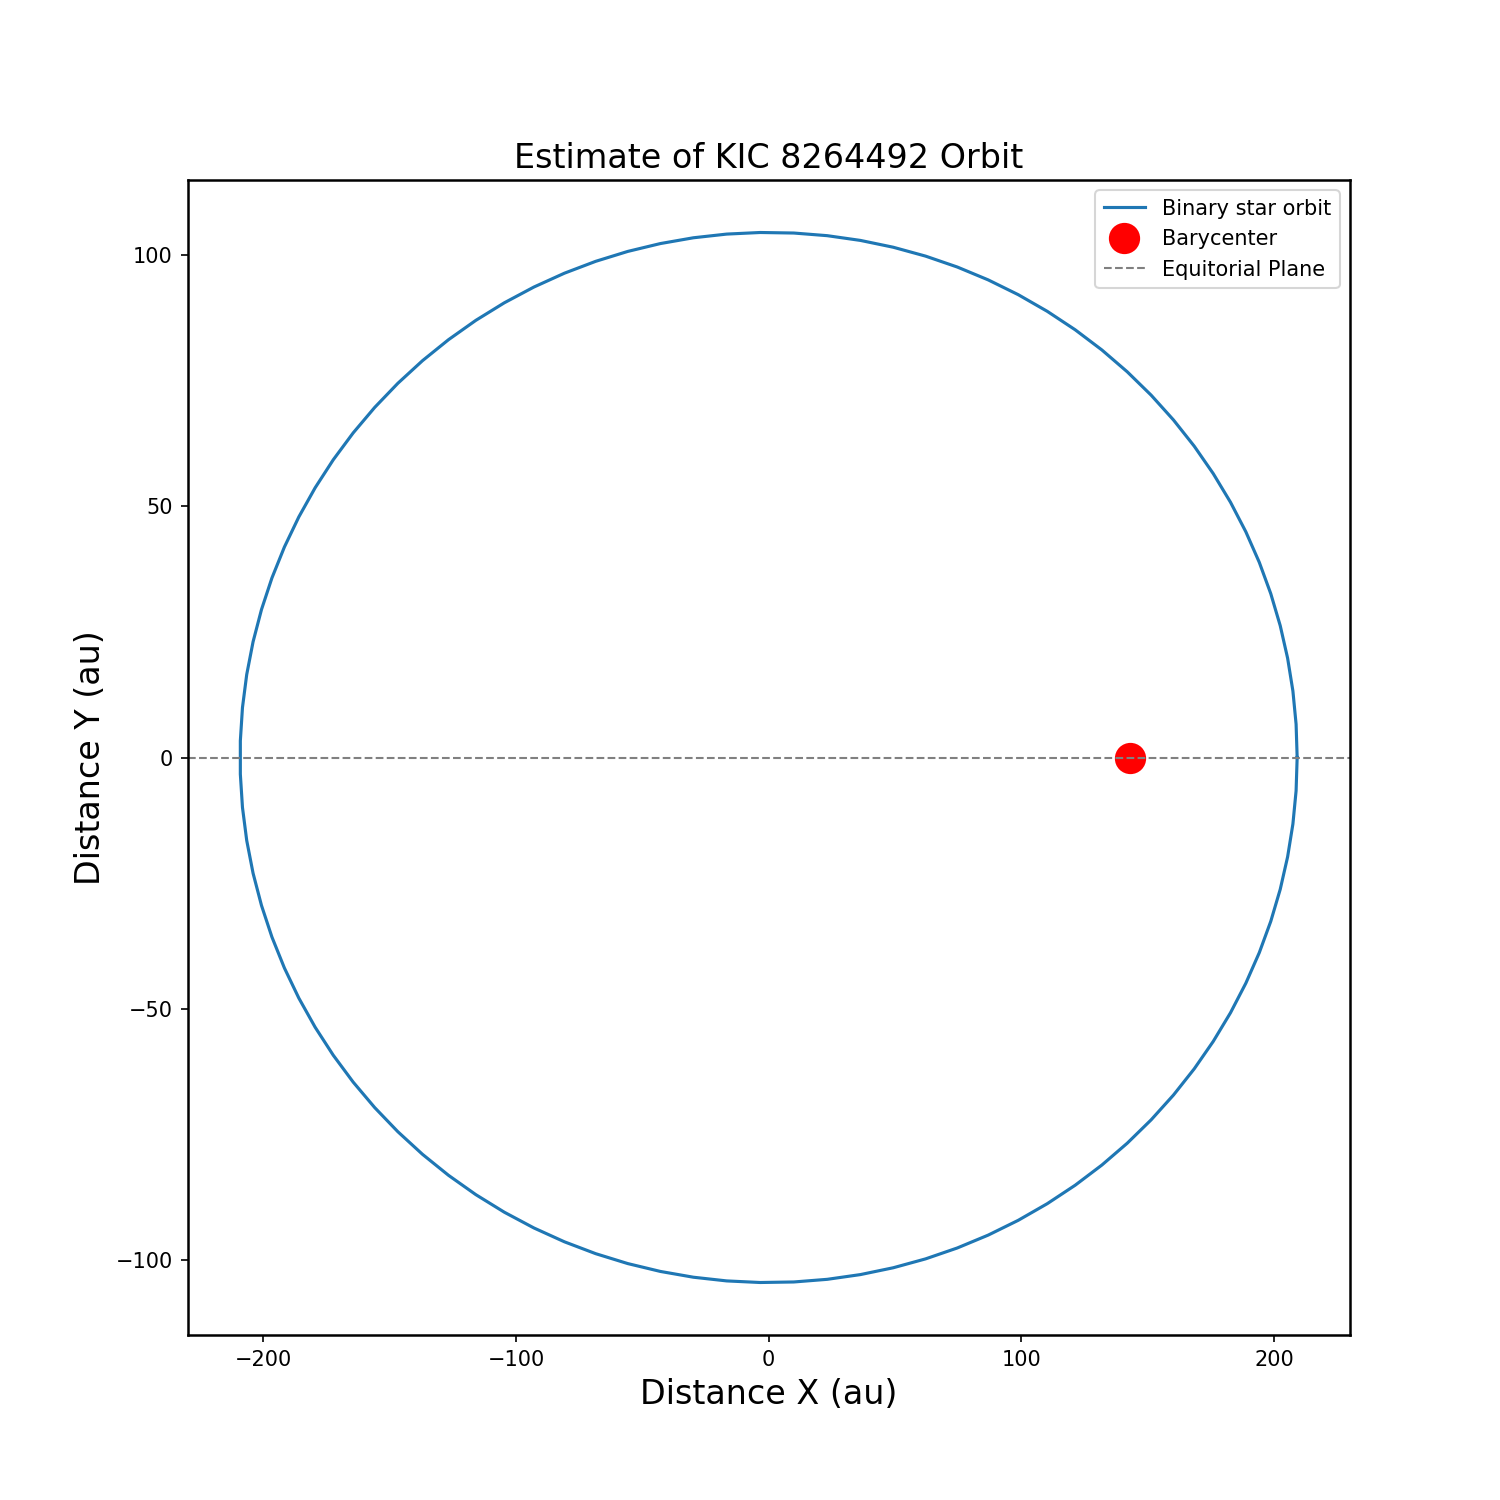
\includegraphics[width=1\linewidth]{orbit.pdf}
      \caption{Need new caption}
      \label{fig:Orbit}
\end{figure}
Also in this figure is an estimate of where the center of mass for the two planets would occur, labelled in the red circle. Since the orbital parameters of the other star in binary is unknown, it is not possible to make a schematic of that orbit.

It is also possible to extract the theoretical light curve from the time delay signal which is shown in Fig \ref{fig:LightcurveOptimized}.
\begin{figure}[H]
    \centering
    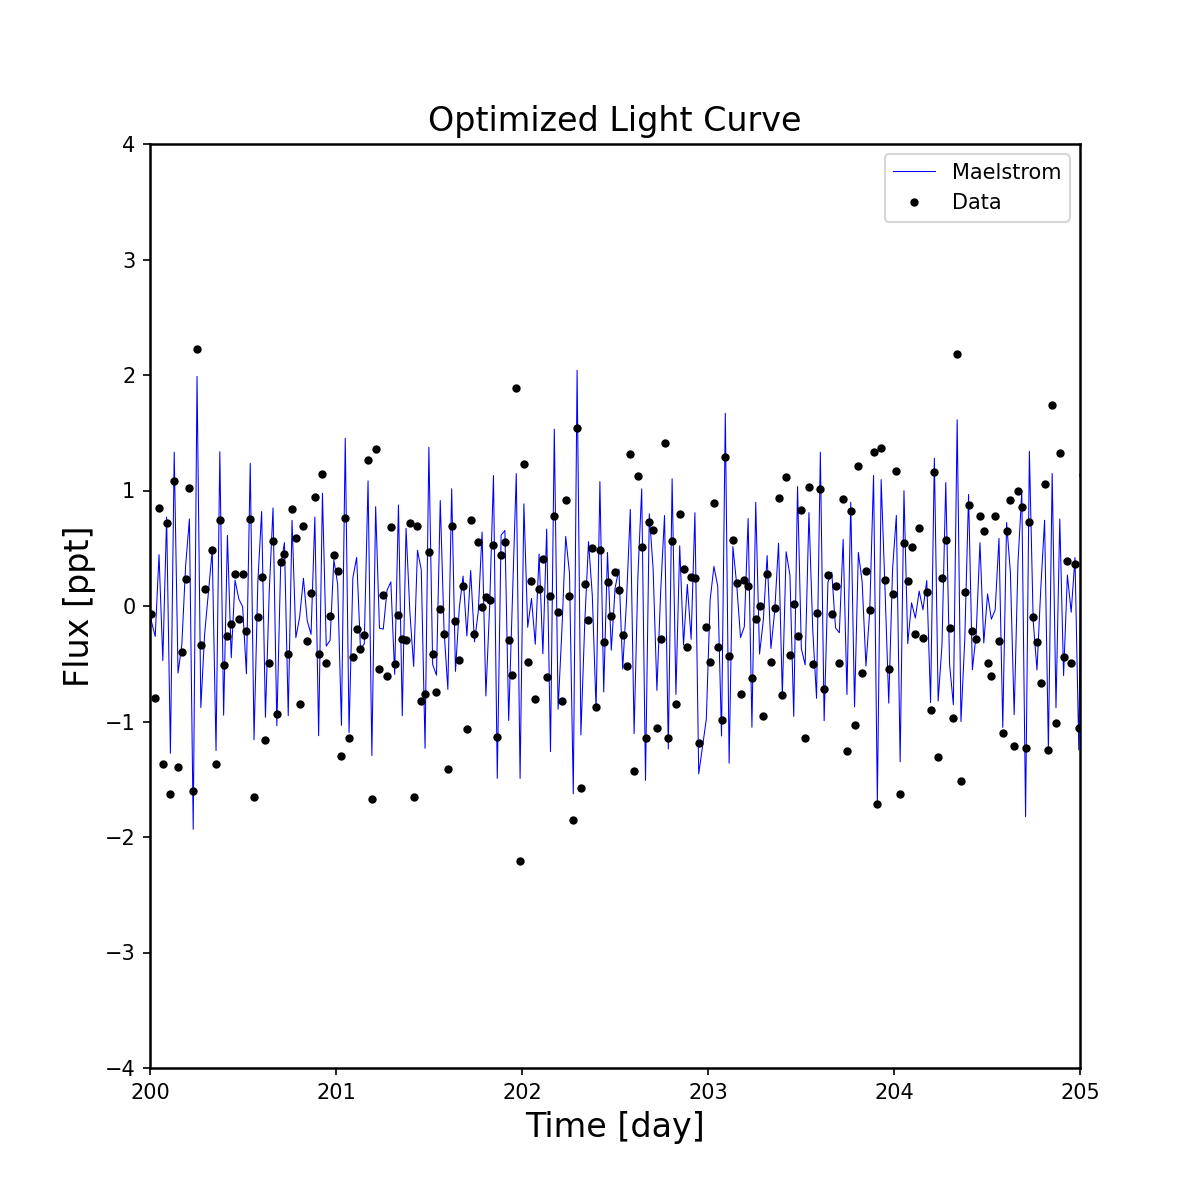
\includegraphics[width=1\linewidth]{lightcurve_opt.pdf}
      \caption{Need new caption}
      \label{fig:LightcurveOptimized}
\end{figure}

It is evident in Fig \ref{fig:LightcurveOptimized} that the original light curve data (black points) agrees really well with the theoretical fit obtained by forward modelling the light curve. Although we can derive this from the time delay signal, this does not provide any further information than the previous light curve signal other than it shows a good correlation with the light curve meaning the model worked

\section{Conclusion}


\bibliography{bibliography}        
\bibliographystyle{unsrt}

\end{document}